\section{مقدمه}
\label{sectio:design:preface}
در این فصل از پژوهش روش طراحی منطق دامنه بر اساس تبادل ناهمگام پیغام ارائه شده است. تلاش شده است تا تطابق طراحی با مدل بازیگر در حد امکان حفظ شود. با توجه به تمرکز این بخش بر روش طراحی منطق دامنه و به هدف ایجاد شفافیت و افزایش قابلیت فهم نکات و الگوهای مطرح شده در روش، تصمیم به استفاده از یک سیستم نمونه به عنوان مثال گرفته شد. کلیه‌ی نکات مطرح شده در ادامه‌ی این بخش در قالب این مثال ارائه خواهند شد. در انتخاب سیستم نمونه نکات ذیل مورد توجه قرار گرفته‌ است:
\begin{enumerate}
\item \textbf{دامنه‌ی سیستم انتخابی:}
رده‌ی دامنه‌ی سیستم انتخاب شده به طور کلی سیستم‌های اطلاعاتی\LTRfootnote{informatiion system} است. اولین دلیل انتخاب این رده این است که در این نوع دامنه همروندی به طور ذاتی وجود ندارد و به همین دلیل زمینه‌ی مقایسه‌ی طراحی بر اساس تبادل ناهمگام با  طراحی‌های شیءگرای ترتیبی فراهم می‌شود. با توجه به اینکه یکی از موارد مقایسه‌ی این نوع طراحی با طراحی شیءگرای ترتیبی تفاوت کارایی این دو رویکرد است، دامنه‌ی انتخاب شده باید در حالت ترتیبی هم قابلیت اضافه شدن همروندی را داشته باشد. سیستم‌های اطلاعاتی از این حیث نیز انتخاب مناسبی محسوب می‌شوند چرا که در اکثر پیاده‌سازی‌های عملیاتی، علیرغم داشتن طراحی ترتیبی، به وسیله‌ی ریسمان‌هایی که وب‌سرورها برای پاسخگویی به درخواست‌های همزمان کاربران ایجاد می‌کنند، دارای خاصیت همروندی نیز می‌گردند. به همین دلیل در بخش ارزیابی می‌توانیم با شبیه‌سازی عملیات وب‌سرورها، کارایی و نیز تغییرپذیری دو نوع طراحی مذکور را ارزیابی و مقایسه کنیم.
 دلیل دیگر این انتخاب بالا بودن میزان آشنایی جامعه‌ی طراحی شیءگرا با این نوع سیستم‌ها و استفاده‌ی گسترده از این نوع سیستم‌ها می‌باشد. شایان ذکر است که سعی شده است در ارائه‌ی الگوها و نکات استخراج شده از این طراحی بر دامنه‌ی انتخاب شده تکیه‌ نشود. دامنه‌ی سیستم نمونه نیز یک سیستم آموزشی انتخاب شده است. با توجه به اینکه استفاده کنندگان این پژوهش جامعه‌ی دانشگاهی هستند، آشنایی این جامعه با سیستم آموزشی دلیل اصلی انتخاب آن بوده است. 
\item \textbf{ بزرگی منطق دامنه:}
از نظر میزان بزرگی سیستم (تعداد کلاس‌ها و موارد کاربرد\LTRfootnote{use cases})،‌  سعی شده منطق حد اقل بزرگی و پیچیدگی را داشته باشد تا ضمن امکان مشاهده‌ی الگوهای مختلف، نیازی به تکرار نکات طراحی برای مولفه‌های متعدد و مشابه نباشد. 
\end{enumerate} 

\section{معرفی یک سیستم آموزش ساده }
\label{section:caseDesign}
همان‌طور که در بخش \ref{sectio:design:preface} ذکر شد،‌ یک سیستم آموزش کوچک به عنوان مدل طراحی انتخاب شده است. در ادامه‌ی این بخش با ارائه‌ی موجودیت\LTRfootnote{entity}‌های اصلی سیستم آموزش و همچنین موارد کاربرد\LTRfootnote{use cases} انتخاب شده، به معرفی این مدل می‌پردازیم.
\subsection{موجودیت‌های اصلی}
 موجودیت‌های اصلی  مدل ابتدایی این سیستم عبارتند از:
\textbf{\textit{دانشجو}}\LTRfootnote{Student}، \textbf{\textit{درس}}\LTRfootnote{Course}، \textbf{\textit{ترم}}\LTRfootnote{Term}، \textbf{\textit{ارائه}}\LTRfootnote{Offering} و \textbf{\textit{سابقه}}\LTRfootnote{Study Record}.\\
در هر \textit{ترم} تحصیلی، تعدادی \textit{ارائه} از دروس مختلف وجود دارد. هر درس می‌تواند \textit{ارائه}های مختلفی داشته باشد. به عنوان مثال درس ریاضی۱ می‌تواند در ترم ۹۰-۹۱-۱سه ارائه‌ی مختلف داشته باشد. دانشجو با اخذ هر ارائه \textit{سابقه}‌ای از آن ارائه را به اسم خود ثبت می‌کند. در این سابقه اطلاعاتی مثل نمره‌ی دانشجو و وضعیت قبول یا مردودی درس در طول ترم ثبت خواهد شد. دروس می‌توانند رابطه‌ی پیش‌نیازی\LTRfootnote{prerequisite} باهم داشته باشند. 
\begin{figure*}
    \begin{center}
	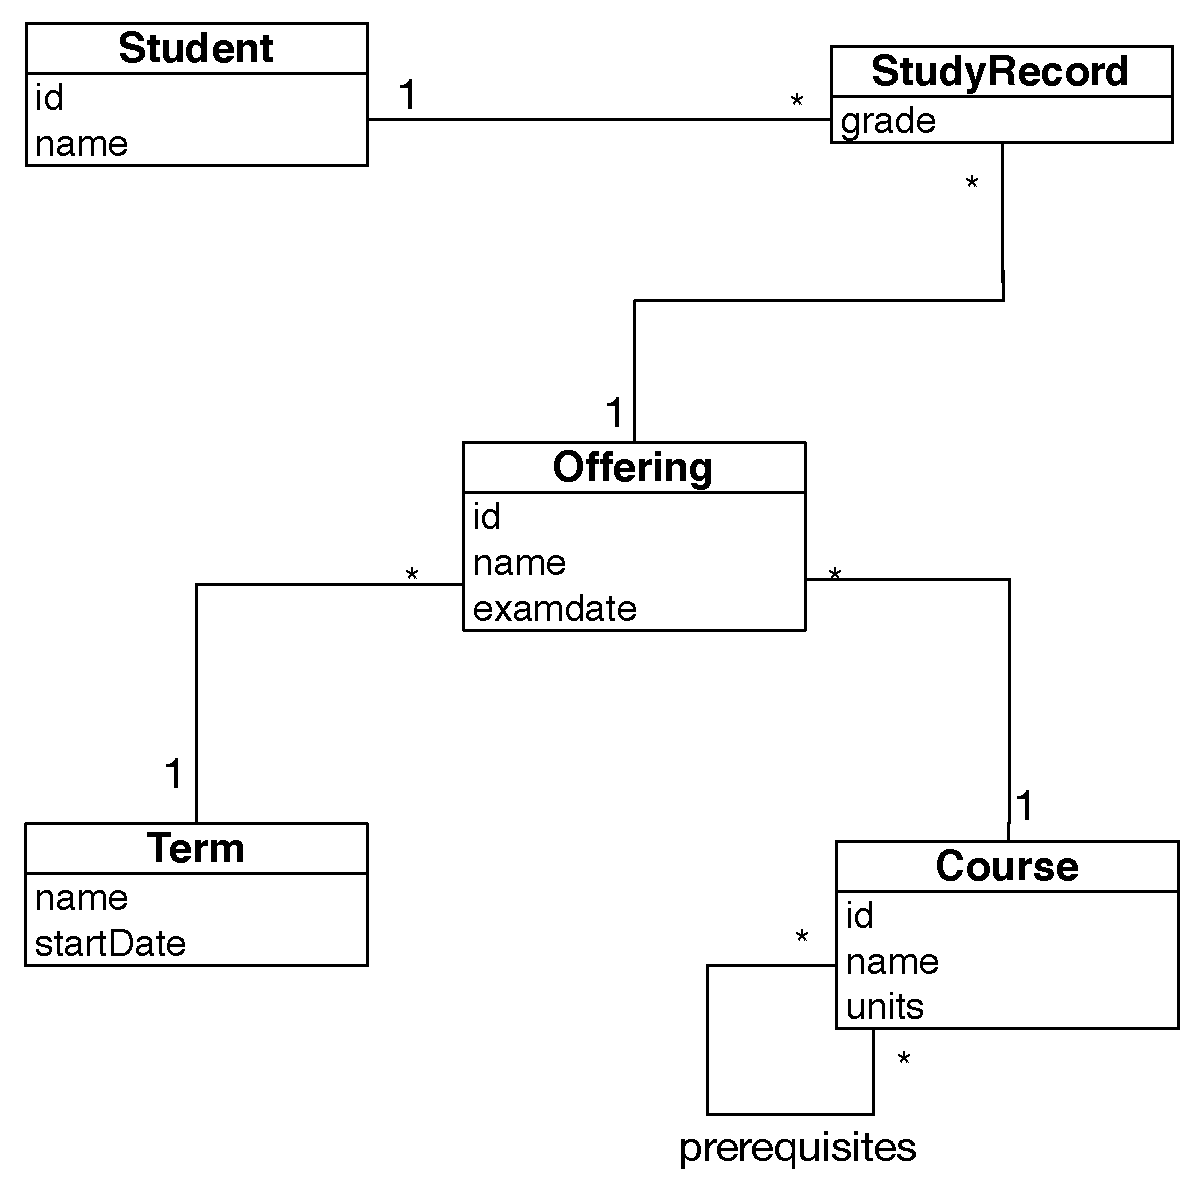
\includegraphics[width=16cm]{4-ProposedFramework/Figures/SimpleClassDiagram.pdf}
    \end{center}
    \caption{\label{fig:edu_class1} نمودار کلاس مدل ابتدای سیستم آموزش ساده }
\end{figure*}
شکل \ref{fig:edu_class1} نمودار کلاس مبتنی بر \textbf{یو‌ام‌ال}\LTRfootnote{UML} سیستم آموزش را نشان می‌دهد. 

%%%%%%%%%%%%%%%%%%%%%%%%%%%%%
%%%%  CHECK COURSE PASSED
%%%%%%%%%%%%%%%%%%%%%%%%%%%%%
\subsection{موارد کاربرد}
در این بخش موارد کاربرد انتخاب شده برای سیستم آموزش معرفی می‌شوند. لازم به تأکید است که علیرغم این که این موارد کاربرد، مرتبط و هماهنگ با موارد کاربرد یک سیستم آموزش واقعی هستند، به هیچ عنوان تمام موارد کاربرد مورد نیاز برای ساختن سیستم واقعی را شامل نمی‌شوند و علاوه‌ بر آن، موارد انتخاب شده دارای جزئیات و دقت کافی برای پوشش فرایند‌های واقعی نیستند. در ادامه‌ی این بخش، هر \gls{مورد کاربرد} در قالب یک جدول توصیفی ارائه شده‌ است.
\begin{table}
\begin{center}
\begin{tabular}{|p{5cm}|p{10cm}|}
	\hline
	\textbf{نام مورد کاربرد} &
کنترل گذراندن موفق درس\\
	\hline
	\textbf{بازیگر(ان)} &
کاربر، سیستم\\
	\hline
	\textbf{شروع می‌شود زمانی که} &
 درخواست مشاهده‌ی وضعیت درس  به سیستم وارد می‌شود.\\
	\hline
	\textbf{پیش‌شرط‌ها} &
ندارد.\\
	\hline
	\textbf{جریان اصلی} &

۱. درخواست مشاهده‌ی وضعیت درس به سیستم وارد می‌شود.\newline
۲. سیستم سابقه‌ی درس مورد نظر در سوابق دانشجو را بررسی می‌کند.\newline
۳. در صورتی که نمره‌ی درس در سابقه بالاتر از ۱۰ یا برابر با ۱۰ باشد سیستم به کاربر جواب مثبت می‌دهد. در غیر این صورت جواب منفی به کاربر اطلاع داده می‌شود.\\
	\hline
%	\textbf{جریان استثنا ۱} &
%۴-ب. کارت کاربر نامعتبر است، پیام خطای کارت نامعتبر است به کاربر نمایش داده شده و تراکنش متوقف می‌شود\\
%	\hline
%	\textbf{جریان استثنا ۲} &
%۴-ج. رمز وارد شده نامعتبر است، پیام خطای رمز نامعتبر است به کاربر نمایش داده شده و تراکنش متوقف می‌شود\\
%	\hline
	\textbf{تمام می‌شود زمانی که} &
نتیجه‌ی درخواست برای کاربر نمایش داده می‌شود.\\
	\hline
%	\textbf{پس شرط‌ها} &
%کاربر موجودی کارت و یا خطای تراکنش را مشاهده کرده است.\\
%	\hline
\end{tabular}
\caption{\label{table:uc_checkpasscourse} توصیف مورد کاربرد کنترل گذراندن موفق درس}
\end{center}
\end{table}
%%%%%%%%%%%%%%%%%%%%%%%%%%%%%
%%%%  CHECK NUM OF UNITS
%%%%%%%%%%%%%%%%%%%%%%%%%%%%%
\begin{table}
\begin{center}
\begin{tabular}{|p{5cm}|p{10cm}|}
	\hline
	\textbf{نام مورد کاربرد} &
محاسبه‌ی تعداد واحد‌های اخذ شده در ترم\footnote{این مورد کاربرد برای بررسی شروط انتخاب واحد استفاده می‌شود. در صورتی که تعداد واحد‌های انتخاب شده در یک ترم  توسط دانشجو بزرگتر از ۲۰ باشد به او اجازه‌ی اخذ دروس بیشتر داده نخواهد شد.}\\
	\hline
	\textbf{بازیگر(ان)} &
کاربر، سیستم\\
	\hline
	\textbf{شروع می‌شود زمانی که} &
درخواست محاسبه‌ی تعداد واحد‌های اخذ شده  توسط یک کاربر در یک ترم به سیستم وارد می‌شود.\\
	\hline
	\textbf{پیش‌شرط‌ها} &
ندارد.\\
	\hline
	\textbf{جریان اصلی} &
۱. درخواست محاسبه‌ی تعداد واحد‌های اخذ شده  توسط یک کاربر در یک ترم، به سیستم وارد می‌شود.\newline
۲. سیستم سوابق تحصیلی دانشجو در ترم مربوطه را بررسی ‌می‌کند. جمع واحد‌های مربوط به هر درس هر سابقه به عنوان پاسخ در نظر گرفته می‌شود. \\
	\hline
%	\textbf{جریان استثنا ۱} &
%۴-ب. کارت کاربر نامعتبر است، پیام خطای کارت نامعتبر است به کاربر نمایش داده شده و تراکنش متوقف می‌شود\\
%	\hline
%	\textbf{جریان استثنا ۲} &
%۴-ج. رمز وارد شده نامعتبر است، پیام خطای رمز نامعتبر است به کاربر نمایش داده شده و تراکنش متوقف می‌شود\\
%	\hline
	\textbf{تمام می‌شود زمانی که} &
نتیجه‌ی درخواست اعلام می‌شود.\\
	\hline
%	\textbf{پس شرط‌ها} &
%کاربر موجودی کارت و یا خطای تراکنش را مشاهده کرده است.\\
%	\hline
\end{tabular}
\caption{\label{table:uc_checknumofunits} توصیف مورد کاربرد محاسبه‌ی تعداد واحد‌های اخذ شده در ترم}
\end{center}
\end{table}

%%%%%%%%%%%%%%%%%%%%%%%%%%%%%
%%%%  CHECK HAS TAKEN COURSE
%%%%%%%%%%%%%%%%%%%%%%%%%%%%%
\begin{table}
\begin{center}
\begin{tabular}{|p{5cm}|p{10cm}|}
	\hline
	\textbf{نام مورد کاربرد} &
بررسی اخذ شدن درس در یک ترم\footnote{به تفاوت بین اخذ و گذراندن درس دقت شود. درس زمانی اخذ شده که سابقه‌ی آن برای دانشجو موجود باشد ولی نمره‌ای برای آن درج نشده باشد. این مورد کاربرد برای جلوگیری از اخذ مجدد درس در زمان انتخاب واحد استفاده می‌شود.}\\
	\hline
	\textbf{بازیگر(ان)} &
سیستم\\
	\hline
	\textbf{شروع می‌شود زمانی که} &
درخواستی به سیستم وارد می‌شود مبنی بر اینکه آیا یک درس در یک ترم تحصیلی توسط دانشجو اخذ شده است یا خیر.\\
	\hline
	\textbf{پیش‌شرط‌ها} &
ندارد.\\
	\hline
	\textbf{جریان اصلی} &
۱. درخواست بررسی اخذ درس در ترم وارد سیستم می‌شود.\newline
۲. سیستم سوابق تحصیلی دانشجو در ترم مربوطه را بررسی ‌می‌کند. اگر سابقه‌ای برای درس مورد نظر وجود داشته باشد که نمره‌ای برای آن وارد نشده پاسخ مثبت می‌دهد. در غیر این صورت پاسخ منفی می‌دهد. \\
	\hline
%	\textbf{جریان استثنا ۱} &
%۴-ب. کارت کاربر نامعتبر است، پیام خطای کارت نامعتبر است به کاربر نمایش داده شده و تراکنش متوقف می‌شود\\
%	\hline
%	\textbf{جریان استثنا ۲} &
%۴-ج. رمز وارد شده نامعتبر است، پیام خطای رمز نامعتبر است به کاربر نمایش داده شده و تراکنش متوقف می‌شود\\
%	\hline
	\textbf{تمام می‌شود زمانی که} &
نتیجه‌ی درخواست اعلام می‌شود.\\
	\hline
%	\textbf{پس شرط‌ها} &
%کاربر موجودی کارت و یا خطای تراکنش را مشاهده کرده است.\\
%	\hline
\end{tabular}
\caption{\label{table:uc_checkcoursetaken} توصیف مورد کاربرد بررسی اخذ درس توسط دانشجو در یک ترم}
\end{center}
\end{table}


%%%%%%%%%%%%%%%%%%%%%%%%%%%%%
%%%%  GPA
%%%%%%%%%%%%%%%%%%%%%%%%%%%%%
\begin{table}
\begin{center}
\begin{tabular}{|p{5cm}|p{10cm}|}
	\hline
	\textbf{نام مورد کاربرد} &
درخواست محاسبه‌ی معدل ترم دانشجو\\
	\hline
	\textbf{بازیگر(ان)} &
کاربر\\
	\hline
	\textbf{شروع می‌شود زمانی که} &
درخواست محاسبه‌ی معدل ترم وارد سیستم می‌شود.\\
	\hline
	\textbf{پیش‌شرط‌ها} &
دانشجو و ترم در سیستم تعریف شده باشند.\\
	\hline
	\textbf{جریان اصلی} &
۱. درخواست محاسبه‌ی معدل دانشجو در ترم مربوطه وارد سیستم می‌شود.\newline
۲. سیستم سوابق تحصیلی دانشجو در ترم مربوطه را بررسی ‌می‌کند. معدل ترم با توجه به نمرات اخذ شده و تعداد واحد هر درس محاسبه و اعلام می‌شود. در صورتی که نمره‌ی درس سابقه‌ای وارد نشده باشد، درس مربوطه در محاسبه‌ی معدل لحاظ نمی‌گردد.\\
	\hline
\textbf{جریان استثنا ۱} &
در صورتی که دانشجو هیچ واحدی در ترم جاری اخذ نکرده باشد پیغام خطای مناسب صادر می‌شود.\\
	\hline
%	\textbf{جریان استثنا ۲} &
%۴-ج. رمز وارد شده نامعتبر است، پیام خطای رمز نامعتبر است به کاربر نمایش داده شده و تراکنش متوقف می‌شود\\
%	\hline
	\textbf{تمام می‌شود زمانی که} &
معدل دانشجو اعلام می‌شود یا خطای مناسب صادر می‌گردد.\\
	\hline
%	\textbf{پس شرط‌ها} &
%کاربر موجودی کارت و یا خطای تراکنش را مشاهده کرده است.\\
%	\hline
\end{tabular}
\caption{\label{table:uc_gpa} توصیف مورد کاربرد محاسبه‌ی معدل یک دانشجو در یک ترم}
\end{center}
\end{table}

%%%%%%%%%%%%%%%%%%%%%%%%%%%%%
%%%%  Take Course
%%%%%%%%%%%%%%%%%%%%%%%%%%%%%
\begin{table}
\begin{center}
\begin{tabular}{|p{4cm}|p{12cm}|}
	\hline
	\textbf{نام مورد کاربرد} &
درخواست اخذ یک ارائه در یک ترم\\
	\hline
	\textbf{بازیگر(ان)} &
کاربر\\
	\hline
	\textbf{شروع می‌شود زمانی که} &
درخواست محاسبه‌ی معدل ترم وارد سیستم می‌شود.\\
	\hline
	\textbf{پیش‌شرط‌ها} &
۱. دانشجو و ترم در سیستم تعریف شده باشند و ارائه‌ی مورد نظر مربوط به ترم انتخاب شده باشد\newline
۲. ‌انتخاب واحد در ترم امکانپذیر باشد. (رجوع کنید به جداول \ref{table:uc_enableofferings}و\ref{table:uc_disableofferings})\\
	\hline
	\textbf{جریان اصلی} &
۱. سیستم کنترل می‌کند که دانشجو در ترم‌های قبل این درس را نگذرانده باشد.\newline
۲. سیستم کنترل می‌کند که دانشجو در ترم‌ جاری این درس را اخذ نکرده باشد.\newline
۳. سیستم کنترل می‌کند که دانشجو تمام پیش‌نیاز‌های این درس را با موفقیت گذرانده باشد.\newline
۴. سیستم کنترل می‌کند که تعداد واحد‌های اخذ شده توسط دانشجو در این ترم پس از اخذ این درس بیشتر از ۲۰ نشود.\newline
۵. سیستم یک سابقه از ارائه‌ی انتخاب شده برای دانشجو تشکیل می‌دهد و آن را در سوابق دانشجو ثبت می‌کند.\\
	\hline
\textbf{جریان استثنا ۱} &
در صورتی که دانشجو قبلا این درس را گذرانده باشد، خطای ''درس انتخاب شده قبلاً گذرانده شده است`` صادر می‌شود.\\
	\hline
\textbf{جریان استثنا ۲} &
در صورتی که دانشجو در ترم جاری این درس را اخذ کرده باشد، خطای ''این درس در ترم جاری قبلاً اخذ شده است`` صادر می‌شود.\\
	\hline
\textbf{جریان استثنا ۳} &
در صورتی که دانشجو یکی از پیش‌نیاز‌های درس‌ را نگذرانده باشد، خطای ''انتخاب بیشتر از ۲۰ واحد در ترم مجاز نمی‌باشد`` صادر می‌شود.\\
	\hline
\textbf{جریان استثنا ۴} &
در صورتی که تعداد واحد‌های اخذ شده توسط دانشجو در این ترم پس از اخذ این درس بیشتر از ۲۰ شود، خطای ''انتخاب بیشتر از ۲۰ واحد در ترم مجاز نمی‌باشد`` صادر می‌شود.\\
	\hline
	\textbf{تمام می‌شود زمانی که} &
سابقه‌ی جدید در سوابق دانشجو ثبت می‌شود و یا خطای مناسب صادر می‌گردد.\\
	\hline
%	\textbf{پس شرط‌ها} &
%کاربر موجودی کارت و یا خطای تراکنش را مشاهده کرده است.\\
%	\hline
\end{tabular}
\caption{\label{table:uc_takecoure} توصیف مورد کاربرد اخذ یک ارائه توسط یک دانشجو در یک ترم}
\end{center}
\end{table}

%%%%%%%%%%%%%%%%%%%%%%%%%%%%%
%%%%  DISABLE_TERM_OFFERINGS
%%%%%%%%%%%%%%%%%%%%%%%%%%%%%
\begin{table}
\begin{center}
\begin{tabular}{|p{5cm}|p{10cm}|}
	\hline
	\textbf{نام مورد کاربرد} &
درخواست غیر فعال کردن ارائه‌های یک ترم برای انتخاب واحد\\
	\hline
	\textbf{بازیگر(ان)} &
کاربر(مدیر سیستم)\\
	\hline
	\textbf{شروع می‌شود زمانی که} &
درخواست غیرفعال کردن ارائه‌های یک ترم وارد سیستم می‌شود.\\
	\hline
	\textbf{پیش‌شرط‌ها} &
 ترم در سیستم تعریف شده باشند.\\
	\hline
	\textbf{جریان اصلی} &
۱. درخواست غیر فعال کردن ارائه‌های یک ترم وارد سیستم می‌شود.\newline
۲.سیستم تمام ارائه‌های یک ترم را غیرفعال می‌کند.\\
	\hline
	\textbf{تمام می‌شود زمانی که} &
تمام ارائه‌های ترم برای انتخاب واحد غیرفعال می‌شوند.\\
	\hline
	\textbf{پس شرط‌ها} &
انتخاب واحد در ترم امکان پذیر نیست.\\
	\hline
\end{tabular}
\caption{\label{table:uc_disableofferings} توصیف مورد کاربرد غیرفعال کردن ارائه‌های یک ترم برای انتخاب واحد}
\end{center}
\end{table}

%%%%%%%%%%%%%%%%%%%%%%%%%%%%%
%%%%  ENABLE_TERM_OFFERINGS
%%%%%%%%%%%%%%%%%%%%%%%%%%%%%
\begin{table}
\begin{center}
\begin{tabular}{|p{5cm}|p{10cm}|}
	\hline
	\textbf{نام مورد کاربرد} &
درخواست فعال کردن ارائه‌های یک ترم برای انتخاب واحد\\
	\hline
	\textbf{بازیگر(ان)} &
کاربر(مدیر سیستم)\\
	\hline
	\textbf{شروع می‌شود زمانی که} &
درخواست فعال کردن ارائه‌های یک ترم وارد سیستم می‌شود.\\
	\hline
	\textbf{پیش‌شرط‌ها} &
 ترم در سیستم تعریف شده باشند.\\
	\hline
	\textbf{جریان اصلی} &
۱. درخواست فعال کردن ارائه‌های یک ترم وارد سیستم می‌شود.\newline
۲.سیستم تمام ارائه‌های یک ترم را فعال می‌کند.\\
	\hline
	\textbf{تمام می‌شود زمانی که} &
تمام ارائه‌های ترم برای انتخاب واحدفعال می‌شوند.\\
	\hline
	\textbf{پس شرط‌ها} &
انتخاب واحد در ترم امکان پذیر است.\\
	\hline
\end{tabular}
\caption{\label{table:uc_enableofferings} توصیف مورد کاربرد فعال کردن ارائه‌های یک ترم برای انتخاب واحد}
\end{center}
\end{table}

\newpage
\section{طراحی سیستم آموزش به روش تبادل ناهمگام پیغام}
سلام
\subsection{طراحی بازیگر‌های اصلی}
سلام
\subsection{مورد کاربرد ۱}
سلام
\subsubsection{رویکرد اول}
سلام
\subsubsection{رویکرد دوم}
سلام
\subsubsection{رویکرد نهایی}
سلام
\subsection{مورد کاربرد ۲}
سلام

\section{الگوهای طراحی استخراج شده و نکات مهم}
اینجا یه سری الگو می‌دم و رفرنس می‌دم که اینجا اینو دیدیم.
